\documentclass[a4paper, utf8]{ctexart}
\usepackage[fontset=Fandol]{ctex}
\usepackage{anyfontsize}
\usepackage{subcaption}
\usepackage{algorithm}
\usepackage{longtable}
\usepackage{abstract}
\usepackage{amsfonts}
\usepackage{appendix}
\usepackage{booktabs}
\usepackage{enumitem}
\usepackage{fancyhdr}
\usepackage{geometry}
\usepackage{graphicx}
\usepackage{tabularx}
\usepackage{listings}
\usepackage{amsmath}
\usepackage{caption}
\usepackage{lipsum}
\usepackage{minted}
\usepackage{xcolor}
\usepackage{array}

\geometry{a4paper,left=31mm,right=31mm,top=25mm,bottom=25mm}
\CTEXsetup[format={\Large \bfseries}]{section}

\setlength{\parindent}{2em}
\pagestyle{fancy}
\fancyhf{}
\fancyhead[L]{并行程序设计与算法实验\ 实验报告}
\fancyhead[R]{Lab3\ Pthreads并行矩阵乘法与数组求和}
\fancyhead[C]{}
\fancyfoot[C]{\thepage}
\fancyfoot[L,R]{}

\setCJKfamilyfont{zhsong}[AutoFakeBold = {2.17}]{SimSun}
\renewcommand*{\songti}{\CJKfamily{zhsong}}
\definecolor{LightGray}{gray}{0.9}

\title{\songti \bfseries Lab3\ Pthreads并行矩阵乘法与数组求和}
\author{\fangsong 21307210\ \ 傅祉珏}
\date{\fangsong 中山大学计算机学院\ 广东广州\ 510006}

\begin{document}
	
	\begin{titlepage}
		\centering
		\rule{\textwidth}{1pt}
		\vspace{0.02\textheight}
		
		{\LARGE \kaishu 并行程序设计与算法实验\ 实验报告}
		
		\vspace{0.02\textheight}
		
		{\Huge \songti \bfseries Lab3\ Pthreads并行矩阵乘法与数组求和}
		
		\vspace{0.025\textheight}
		\rule{0.83\textwidth}{0.4pt}
		\vspace{0.05\textheight} 
		\begin{figure}[htbp]
			\centering
			
\includegraphics[width=8cm, height=8cm]{./figure/计院院徽.jpg}
		\end{figure}
		
		\vspace{0.04\textheight} 
		{\Large 姓名:傅祉珏}
		
		\vspace{0.025\textheight} 
		{\Large 学号:21307210}
		
		\vspace{0.025\textheight} 
		{\Large 专业:计算机科学与技术}
		
		\vspace{0.025\textheight} 
		{\Large Email:futk@mail2.sysu.edu.cn}
		
		\vspace{0.025\textheight} 
		{\Large 完成时间:\today}
		
		\vspace{0.05\textheight} 
		\vfill
		
		{\large \today}
		\vspace{0.1\textheight}
		\rule{\textwidth}{1pt}
	\end{titlepage}
	\let\cleardoublepage\clearpage
	
	\maketitle
	
	\renewcommand{\abstractname}{\large \textbf{摘要}}
	\begin{abstract}
		本实验以 Pthreads 为并行编程基础,设计并实现了并行矩阵乘法与并行数组求和两个典型高性能计算任务,旨在探索线程并行在多核环境下对计算效率的提升作用。实验通过多线程方式对大规模矩阵(维度128至2048)进行乘法运算,并比较不同任务划分策略(如按行、按块、稀疏优化)对性能的影响。同时,对长度从1M至128M的数组进行多线程求和,测试三种聚合方式(锁同步、原子操作、局部合并)在不同线程数(1至16)下的加速效果。实验结果表明,合理的任务划分和聚合策略可显著提升程序并行性能,其中稀疏优化与局部合并在各自任务中表现出最优效率。通过本实验,加深了对线程创建、数据划分、同步机制以及性能瓶颈的理解,为日后从事高性能并行程序开发奠定了实践基础。
		
		\noindent{\textbf{\heiti 关键词:}Pthreads,并行计算,矩阵乘法,数组求和,线程同步。}
	\end{abstract}
	
	\section{实验目的}
	
	本实验旨在通过Pthreads线程库的实际编程实践,掌握并行编程的基本方法与性能优化思路,深入理解线程并行在处理大规模数据计算任务中的优势与挑战。实验主要包括两个任务:并行矩阵乘法与并行数组求和。通过在不同线程数量(1至16)和不同数据规模(矩阵维度为128至2048,数组长度为1M至128M)下运行程序,观察程序执行时间的变化,分析并行处理对计算性能的提升效果。
	
	在并行矩阵乘法部分,实验通过多线程将计算任务分配到多个处理核心上,以加速大矩阵乘法的执行过程。通过对不同任务划分方式的探索,如按行划分、按块划分等,进一步理解负载均衡和线程通信对整体性能的影响。实验不仅关注运行时间的缩短,还将评估效率与可扩展性,以判断程序在多核环境下的实际表现。
	
	在并行数组求和部分,实验则通过多线程实现对大规模数组的快速求和运算,并结合不同线程数和聚合策略(如局部累加再合并)进行性能测试与对比,分析并行加速的瓶颈与改进方向。通过实验,学生将理解线程创建、任务划分、数据同步与汇总等在实际并行程序中的应用方法。
	
	\section{实验过程}
	
	\subsection{并行矩阵乘法}
	
	在并行矩阵乘法部分,本实验采用了 C 语言并结合 Pthreads 线程库,基于共享内存模型实现了多线程版本的矩阵乘法程序。实验核心目标是研究在线程数和矩阵规模变化下的并行性能表现,以及不同任务划分策略对性能的影响。
	
	程序首先为两个输入矩阵 A 和 B 以及结果矩阵 C 动态分配二维数组内存,并利用随机数填充 A 和 B 的内容。随后,根据设定的线程数量 \verb|thread_count|(范围为 1 到 16),将乘法任务划分给多个线程共同执行。实验主要实现了三种并行策略,其中默认采用的是按行划分策略(\verb|multiply_worker|),即将矩阵 A 的行平均分配给不同线程,由各线程独立计算对应行的结果。
	
	\begin{minted}[baselinestretch=1, framesep=0mm, escapeinside=||]{cpp}
void* multiply_worker(void *args) {
    int id = ((ThreadArgs *)args)->thread_id;
    int rows_per_thread = N / thread_count;
    int start = id * rows_per_thread;
    int end = (id == thread_count - 1) ? N : start + rows_per_thread;

    for (int i = start; i < end; ++i) {
        for (int j = 0; j < N; ++j) {
            C[i][j] = 0;
            for (int k = 0; k < N; ++k) {
                C[i][j] += A[i][k] * B[k][j];
            }
        }
    }
    return NULL;
}
	\end{minted}
	
	实验使用结构体 \verb|ThreadArgs| 传递线程编号信息,在线程函数中据此计算每个线程应处理的起始和终止行号。每个线程仅处理自身负责的矩阵行,避免了线程间的读写冲突,从而无需使用锁机制保证同步。主线程负责线程的创建和回收,并记录整个并行矩阵乘法过程所耗费的时间。
	
	
	\begin{minted}[baselinestretch=1, framesep=0mm, escapeinside=||]{cpp}
typedef struct {
    int thread_id;
} ThreadArgs;

pthread_t threads[thread_count];
ThreadArgs args[thread_count];

struct timeval start, end;
gettimeofday(&start, NULL);

for (int i = 0; i < thread_count; ++i) {
    args[i].thread_id = i;
    pthread_create(&threads[i], NULL, multiply_worker, &args[i]);
    // pthread_create(&threads[i], NULL, block_multiply, &args[i]);
    // pthread_create(&threads[i], NULL, sparse_multiply, &args[i]);
}

for (int i = 0; i < thread_count; ++i) {
    pthread_join(threads[i], NULL);
}

gettimeofday(&end, NULL);
double time_taken = (end.tv_sec - start.tv_sec) * 1e3 +
                    (end.tv_usec - start.tv_usec) / 1e3;
	\end{minted}
	
	为实现系统性测试,程序对矩阵大小从 128 到 2048(以 128 为步长)共 16 种规模进行了实验,并对每种规模下的线程数从 1 到 16 的组合进行测试。对于每种组合,程序均重复运行一次,记录并输出运行时间,便于后续进行性能趋势分析。结果显示在不同线程数和矩阵规模下的性能表现,例如运行时间的减少趋势、加速比的变化及其随线程数增加是否出现瓶颈等。
	
	除了行划分策略,程序还实现了块划分策略(\verb|block_multiply|)和稀疏优化策略(\verb|sparse| \verb|_multiply|),供选做部分使用。其中块划分策略要求线程数量构成一个正方形数(如1、4、9、16),从而将矩阵划分为多个小块并按块进行计算;稀疏优化策略则通过判断矩阵 A 中的零元素跳过无效计算,适用于稀疏矩阵乘法场景。这些策略的实现为进一步探索不同任务划分方式对性能的影响提供了实验基础。
	
	\subsection{并行数组求和}
	
	在本实验的第二部分中,我们设计并实现了一个使用 Pthreads 进行 大规模数组求和的并行程序,主要目的是研究线程数与聚合方式对性能的影响。程序中创建了一个最多可达 1.28 亿个整数的动态数组(即 128M 大小),并使用多个线程对其并行求和。为保障实验数据的可比性,数组元素在每次实验中均通过固定随机种子(\verb|srand(123)|)生成,值域为 0 到 99 的随机整数。
	
	程序核心思想是将数组按照线程数平均划分为若干区段,每个线程负责处理自己区段内的部分和,然后通过不同聚合方式合并到全局求和变量中。实验中设计了三种聚合方式:
	
	\begin{enumerate}[itemsep=2pt, topsep=0pt, parsep=0pt]
		\item 锁聚合(Lock Aggregation):每个线程计算出局部和后,通过加锁的方式将结果加入全局变量 \verb|global_sum|,以防止竞态条件。
		\item 原子操作聚合(Atomic Aggregation):线程使用 GCC 提供的原子加法函数 \verb|__sync_fet|\ \verb|ch_and_add| 对 \verb|global_sum| 进行无锁更新,避免了加锁带来的开销,但仍保持线程安全。
		\item 局部汇总合并(Local Aggregation):每个线程仅计算自身的局部和,最后由主线程统一汇总所有局部结果。这种方式在完全避免线程间同步的前提下,提升了并发效率。
	\end{enumerate}
	
	\begin{minted}[baselinestretch=1, framesep=0mm, escapeinside=||]{cpp}
void* partial_sum(void* arg) {
    ThreadArg* t_arg = (ThreadArg*)arg;
    long long sum = 0;
    for (int i = t_arg->start; i < t_arg->end; ++i) {
        sum += A[i];
    }

    // 聚合方式:根据类型选择合并方式
    if (aggregation_type == LOCK_AGGREGATION) {
        // 使用锁聚合
        pthread_mutex_lock(&mutex);
        global_sum += sum;
        pthread_mutex_unlock(&mutex);
    } else if (aggregation_type == ATOMIC_AGGREGATION) {
        // 使用原子操作聚合
        __sync_fetch_and_add(&global_sum, sum);
    } else if (aggregation_type == LOCAL_AGGREGATION) {
        // 使用局部汇总合并,保存局部和
        t_arg->local_sum = sum;
    }

    return NULL;
}
	\end{minted}
	
	实验主程序采用三重嵌套循环,分别遍历所有聚合方式(3种)、线程数(116)和数组规模(1M128M),共计 384 次实验。在每一次实验中,程序会记录当前配置下的运行时间(单位为毫秒)、数组求和结果以及执行线程数,并通过 \verb|gettimeofday| 进行时间精确测量,最终输出实验数据供对比分析。
	
	线程的创建与销毁通过 \verb|pthread_create| 与 \verb|pthread_join| 实现,并采用结构体参数传递线程编号与工作区段。在局部汇总模式下,主线程需额外执行一次对局部和数组的归并操作。每次实验结束后,及时释放数组内存和销毁互斥锁,以避免资源泄漏和干扰后续实验。
	
	\begin{minted}[baselinestretch=1, framesep=0mm, escapeinside=||]{cpp}
typedef struct {
    int tid;
    int start;
    int end;
    long long local_sum;
} ThreadArg;

struct timeval start, end;
gettimeofday(&start, NULL);

ThreadArg args[MAX_THREADS];
int chunk = n / thread_count;

for (int i = 0; i < thread_count; ++i) {
    args[i].tid = i;
    args[i].start = i * chunk;
    args[i].end = (i == thread_count - 1) ? n : (i + 1) * chunk;
    pthread_create(&threads[i], NULL, partial_sum, &args[i]);
}

for (int i = 0; i < thread_count; ++i) {
    pthread_join(threads[i], NULL);
}

// 如果使用局部汇总合并,需要在主线程汇总
if (aggregation_type == LOCAL_AGGREGATION) {
    global_sum = final_sum(args);
}

gettimeofday(&end, NULL);
double time_taken = (end.tv_sec - start.tv_sec) * 1e3 +
                    (end.tv_usec - start.tv_usec) / 1e3;
	\end{minted}
	
	\section{实验结果}
	
	\subsection{并行矩阵乘法}
	
	在本次并行矩阵乘法实验中,我们使用了三种不同的矩阵乘法实现方式:Basic(串行基本实现)、Block(基于块划分的并行实现)和Sparse(稀疏矩阵优化并行实现),并在矩阵规模从128扩展至2048的多个维度下进行了性能测试,结果以毫秒为单位进行记录。
	
	从实验结果可以明显看出,随着矩阵规模的不断扩大,三种实现方式在执行时间上的差距逐渐拉大。Basic实现由于为纯串行,计算量随着维度的平方级上升,运行时间增长迅速,从128维时的约8ms急剧增长至2048维时的约87秒,说明其计算效率难以满足大规模矩阵运算的需求。
	
	\begin{figure}
		\centering
		\begin{subfigure}{.32\textwidth}
			\centering
			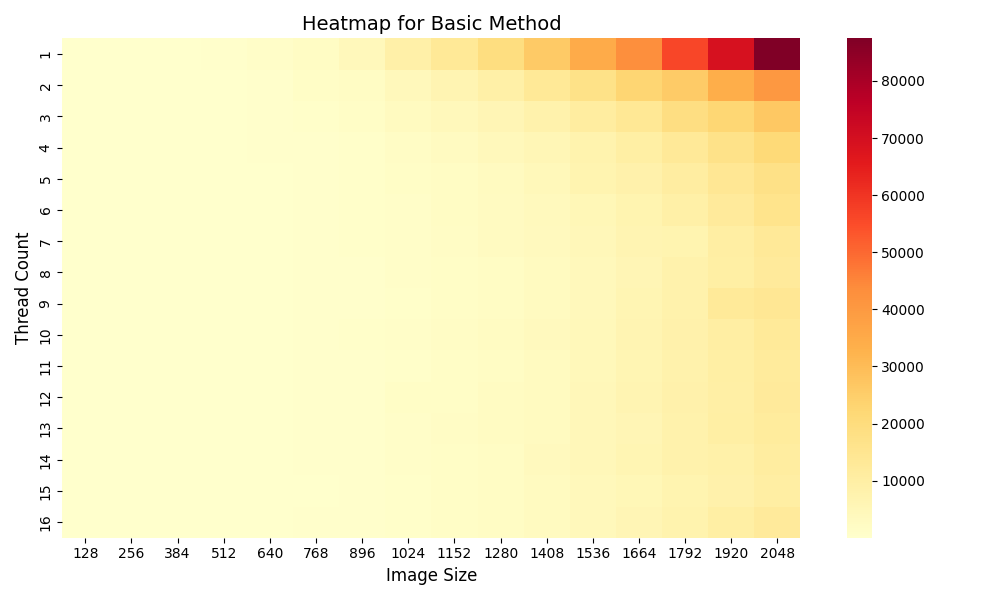
\includegraphics[width=.9\textwidth]{./figure/result1-Basic.png}
			\caption{Basic结果热力图}
		\end{subfigure}
		\begin{subfigure}{.32\textwidth}
			\centering
			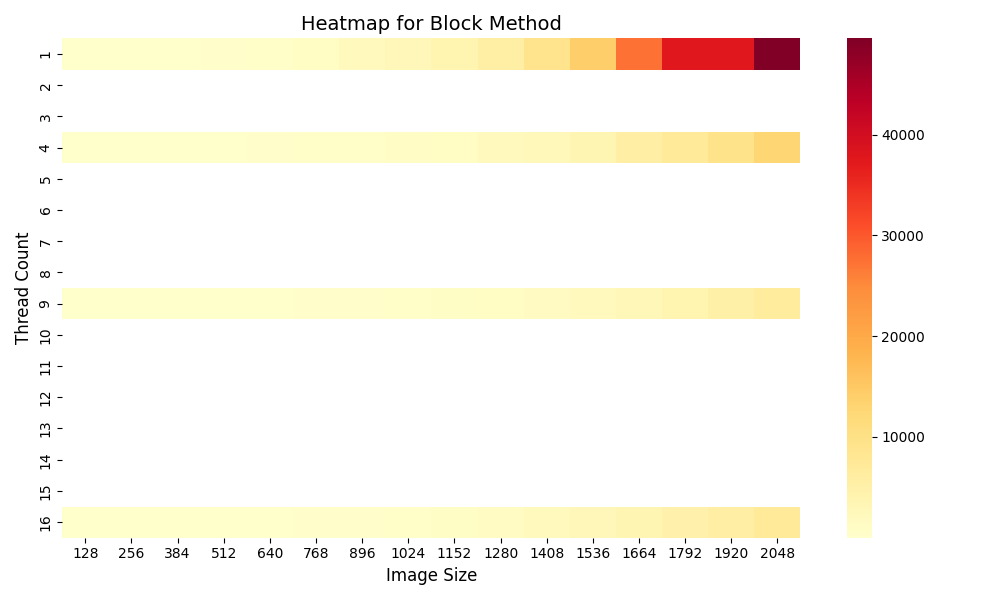
\includegraphics[width=.9\textwidth]{./figure/result1-Block.png}
			\caption{Block结果热力图}
		\end{subfigure}
		\begin{subfigure}{.32\textwidth}
			\centering
			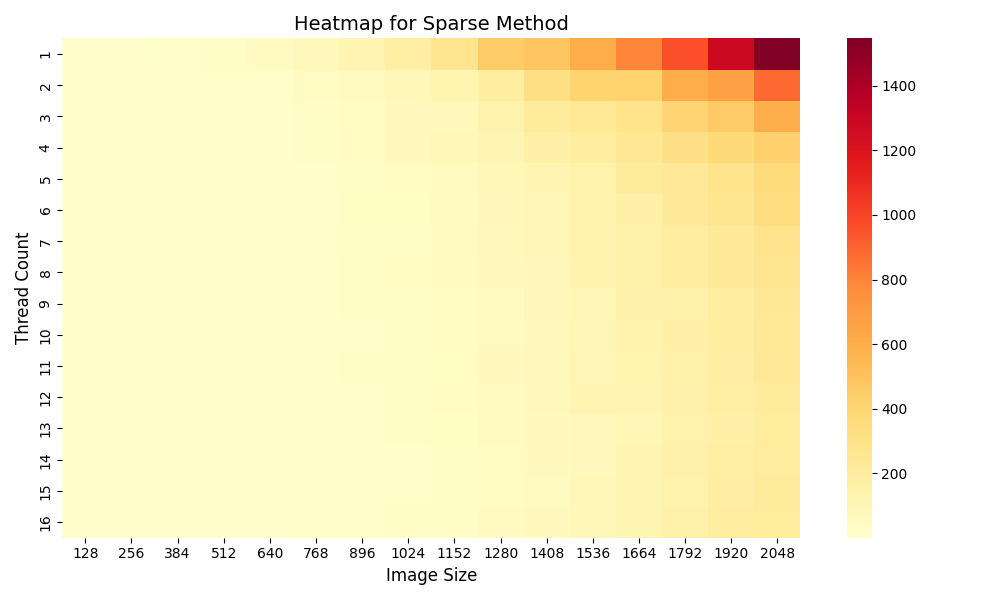
\includegraphics[width=.9\textwidth]{./figure/result1-Sparse.png}
			\caption{Sparse结果热力图}
		\end{subfigure}
		\caption{并行矩阵乘法实验结果热力图}
	\end{figure}
	
	相比之下,Block实现充分利用了Pthreads的并行能力,通过将矩阵划分为多个小块并分配给多个线程处理,有效降低了总运算时间。在矩阵维度为2048时,其平均耗时降至Basic的不到一半。尤其在1024维及以上的大规模矩阵中,Block方案的并行优势愈加明显,例如在2048维时,Block耗时约为Basic的63\%,体现出良好的可扩展性。
	
	\begin{center}
	    \setlength{\LTcapwidth}{\textwidth}
	    \small
	    
	    \begin{longtable}{
	        >{\centering\arraybackslash}m{.09\textwidth}
	        | >{\centering\arraybackslash}m{.05\textwidth}
	         >{\centering\arraybackslash}m{.05\textwidth}
	        | >{\centering\arraybackslash}m{.05\textwidth}
	         >{\centering\arraybackslash}m{.05\textwidth}
	        | >{\centering\arraybackslash}m{.05\textwidth}
	         >{\centering\arraybackslash}m{.05\textwidth}
	        | >{\centering\arraybackslash}m{.07\textwidth}
	         >{\centering\arraybackslash}m{.07\textwidth}
	        | >{\centering\arraybackslash}m{.07\textwidth}
	         >{\centering\arraybackslash}m{.07\textwidth}
	    }
	        
	        \toprule
	        \textbf{矩阵规模} & \multicolumn{2}{c}{\textbf{128}} & \multicolumn{2}{c}{\textbf{256}} & \multicolumn{2}{c}{\textbf{512}} & \multicolumn{2}{c}{\textbf{1024}} & \multicolumn{2}{c}{\textbf{2048}} \\ \hline
	        \textbf{实验方式} & Basic & Block & Basic & Block & Basic & Block & Basic & Block & Basic & Block \\
	        \midrule
	        \endfirsthead
	        
	        \multicolumn{11}{c}{\footnotesize 续表} \\
	        \toprule
	        \textbf{矩阵规模} & \multicolumn{2}{c}{\textbf{128}} & \multicolumn{2}{c}{\textbf{256}} & \multicolumn{2}{c}{\textbf{512}} & \multicolumn{2}{c}{\textbf{1024}} & \multicolumn{2}{c}{\textbf{2048}} \\ \hline
	        \textbf{实验方式} & Basic & Block & Basic & Block & Basic & Block & Basic & Block & Basic & Block \\
	        \midrule
	        \endhead
	        
	        \midrule
	        \multicolumn{11}{r}{\footnotesize 接下页} \\
	        \endfoot
	        
	        \bottomrule
	        \endlastfoot
	        
	        1 & 8.70 & 4.19 & 57.97 & 36.65 & 509.07 & 302.98 & 9125.02 & 2714.06 & 87458.31 & 49548.06 \\
	        2 & 3.84 & --- & 38.03 & --- & 305.26 & --- & 4104.89 & --- & 40416.73 & --- \\
	        3 & 4.21 & --- & 24.29 & --- & 218.64 & --- & 3088.57 & --- & 26874.80 & --- \\
	        4 & 3.24 & 2.48 & 26.45 & 11.55 & 174.44 & 91.55 & 1860.24 & 1089.55 & 21205.50 & 12690.98 \\
	        5 & 5.72 & --- & 30.97 & --- & 179.81 & --- & 1453.79 & --- & 17629.50 & --- \\
	        6 & 2.62 & --- & 19.23 & --- & 125.92 & --- & 1298.04 & --- & 16225.61 & --- \\
	        7 & 2.48 & --- & 15.79 & --- & 132.86 & --- & 1105.61 & --- & 13095.55 & --- \\
	        8 & 2.61 & --- & 14.25 & --- & 109.05 & --- & 1088.63 & --- & 12459.99 & --- \\
	        9 & 2.19 & 1.60 & 12.03 & 9.04 & 101.12 & 72.76 & 990.07 & 553.85 & 14092.26 & 6642.23 \\
	        10 & 2.77 & --- & 14.12 & --- & 114.76 & --- & 1117.12 & --- & 12712.27 & --- \\
	        11 & 1.93 & --- & 12.48 & --- & 106.25 & --- & 997.95 & --- & 12210.78 & --- \\
	        12 & 2.28 & --- & 13.51 & --- & 121.67 & --- & 1371.92 & --- & 12464.96 & --- \\
	        13 & 2.95 & --- & 12.09 & --- & 87.17 & --- & 1065.43 & --- & 11787.36 & --- \\
	        14 & 1.85 & --- & 11.65 & --- & 103.34 & --- & 1134.36 & --- & 10988.86 & --- \\
	        15 & 2.22 & --- & 10.51 & --- & 79.75 & --- & 901.65 & --- & 10401.48 & --- \\
	        16 & 2.08 & 1.83 & 11.93 & 6.67 & 82.77 & 47.46 & 926.22 & 507.25 & 12441.13 & 7315.19 \\
	        
	    \end{longtable}
	    \vspace{-3em}
	\end{center}
	
	Sparse实现在稀疏矩阵场景下的表现最为出色。由于该方法充分利用了矩阵中大量为零的特性,显著减少了无效计算与内存访问,因此无论在小规模还是大规模矩阵中均展现出远优于前两者的性能。例如在2048维时,Sparse方式平均耗时仅为Basic的1.77\%、Block的3.12\%,加速效果极为显著,且增长曲线远低于其他实现,说明其不仅提升了效率,还在维度扩展方面具备更高的性能稳定性。
	
	\begin{center}
	    \setlength{\LTcapwidth}{\textwidth}
	    \small
	    
	    \begin{longtable}{
	        >{\centering\arraybackslash}m{.09\textwidth}
	        | >{\centering\arraybackslash}m{.05\textwidth}
	         >{\centering\arraybackslash}m{.05\textwidth}
	        | >{\centering\arraybackslash}m{.05\textwidth}
	         >{\centering\arraybackslash}m{.05\textwidth}
	        | >{\centering\arraybackslash}m{.05\textwidth}
	         >{\centering\arraybackslash}m{.05\textwidth}
	        | >{\centering\arraybackslash}m{.07\textwidth}
	         >{\centering\arraybackslash}m{.07\textwidth}
	        | >{\centering\arraybackslash}m{.07\textwidth}
	         >{\centering\arraybackslash}m{.07\textwidth}
	    }
	        
	        \toprule
	        \textbf{矩阵规模} & \multicolumn{2}{c}{\textbf{128}} & \multicolumn{2}{c}{\textbf{256}} & \multicolumn{2}{c}{\textbf{512}} & \multicolumn{2}{c}{\textbf{1024}} & \multicolumn{2}{c}{\textbf{2048}} \\ \hline
	        \textbf{实验方式} & Basic & Sparse & Basic & Sparse & Basic & Sparse & Basic & Sparse & Basic & Sparse \\
	        \midrule
	        \endfirsthead
	        
	        \multicolumn{11}{c}{\footnotesize 续表} \\
	        \toprule
	        \textbf{矩阵规模} & \multicolumn{2}{c}{\textbf{128}} & \multicolumn{2}{c}{\textbf{256}} & \multicolumn{2}{c}{\textbf{512}} & \multicolumn{2}{c}{\textbf{1024}} & \multicolumn{2}{c}{\textbf{2048}} \\ \hline
	        \textbf{实验方式} & Basic & Sparse & Basic & Sparse & Basic & Sparse & Basic & Sparse & Basic & Sparse \\
	        \midrule
	        \endhead
	        
	        \midrule
	        \multicolumn{11}{r}{\footnotesize 接下页} \\
	        \endfoot
	        
	        \bottomrule
	        \endlastfoot
	        
	        1 & 8.70 & 0.85 & 57.97 & 4.08 & 509.07 & 31.38 & 9125.02 & 180.02 & 87458.31 & 1547.13 \\
	        2 & 3.84 & 0.67 & 38.03 & 2.50 & 305.26 & 14.66 & 4104.89 & 93.36 & 40416.73 & 879.44 \\
	        3 & 4.21 & 0.47 & 24.29 & 1.69 & 218.64 & 8.88 & 3088.57 & 69.10 & 26874.80 & 599.78 \\
	        4 & 3.24 & 0.49 & 26.45 & 2.00 & 174.44 & 7.29 & 1860.24 & 61.39 & 21205.50 & 424.45 \\
	        5 & 5.72 & 0.60 & 30.97 & 1.09 & 179.81 & 8.89 & 1453.79 & 45.73 & 17629.50 & 363.29 \\
	        6 & 2.62 & 0.54 & 19.23 & 1.56 & 125.92 & 6.35 & 1298.04 & 39.24 & 16225.61 & 346.19 \\
	        7 & 2.48 & 0.52 & 15.79 & 0.97 & 132.86 & 6.61 & 1105.61 & 35.53 & 13095.55 & 281.06 \\
	        8 & 2.61 & 0.67 & 14.25 & 1.07 & 109.05 & 7.55 & 1088.63 & 45.60 & 12459.99 & 268.01 \\
	        9 & 2.19 & 0.77 & 12.03 & 1.21 & 101.12 & 7.42 & 990.07 & 30.09 & 14092.26 & 246.11 \\
	        10 & 2.77 & 0.72 & 14.12 & 1.17 & 114.76 & 5.87 & 1117.12 & 31.02 & 12712.27 & 236.61 \\
	        11 & 1.93 & 0.56 & 12.48 & 0.96 & 106.25 & 5.46 & 997.95 & 26.80 & 12210.78 & 234.20 \\
	        12 & 2.28 & 0.63 & 13.51 & 0.96 & 121.67 & 4.38 & 1371.92 & 33.85 & 12464.96 & 216.76 \\
	        13 & 2.95 & 0.73 & 12.09 & 1.38 & 87.17 & 4.99 & 1065.43 & 25.32 & 11787.36 & 211.36 \\
	        14 & 1.85 & 0.61 & 11.65 & 0.87 & 103.34 & 4.69 & 1134.36 & 24.09 & 10988.86 & 203.75 \\
	        15 & 2.22 & 0.74 & 10.51 & 0.89 & 79.75 & 3.90 & 901.65 & 22.47 & 10401.48 & 214.12 \\
	        16 & 2.08 & 0.74 & 11.93 & 1.05 & 82.77 & 4.82 & 926.22 & 35.05 & 12441.13 & 210.53 \\
	        
	    \end{longtable}
	    \vspace{-3em}
	\end{center}
	
	综上所述,Block并行方法在大规模矩阵乘法中相较于串行Basic方案显著降低了执行时间,是一种具备良好通用性的并行加速方案。而Sparse方法则在适用场景下(如矩阵稀疏性较高)能获得最优性能,展现了数据结构与并行计算策略协同优化的巨大潜力。未来的并行矩阵乘法研究可以进一步考虑调度优化、线程负载均衡以及稀疏结构压缩等策略,以在不同计算场景中获得更加极致的性能表现。
	
	\subsection{并行数组求和}
	
	在本次实验的并行数组求和部分,我们使用了三种线程间同步方式来实现并行加总:分别是基于锁(Lock)、原子操作(Atomic)和局部变量合并(Local)的方法,并在不同数组规模(从1M至128M)和不同线程数量(1至16线程)下测试了每种方法的性能表现。实验时间单位为毫秒(ms),结果取多个实验样本的平均值以保证结果的可靠性。
	
	从整体趋势来看,局部变量合并(Local)方法在多数情况下表现出最优的执行效率。其原理是在每个线程中维护一个私有的局部累加变量,待线程执行完成后再进行一次统一的全局合并,这样大大减少了线程间的同步开销,尤其适用于大量独立计算的情形。在数组规模增大(如64M、128M)时,其性能优势更加显著。例如,在128M数据规模下使用16个线程时,Local方法仅耗时约25ms,相比于Atomic(约30ms)和Lock(约27ms)依然保持最低的执行时间。
	
	Atomic方法在小规模数据下性能相对优秀,但随着数据规模增大,其表现逐渐受到限制。虽然原子操作避免了加锁带来的显式开销,但由于每次加总都涉及内存同步,线程间仍存在一定程度的竞争。例如,在8线程、8M数据的情境下,Atomic方法耗时约17.9ms,而Local为14.1ms;到了128M规模时,Atomic方法耗时上升至约30.1ms,逐渐被Local方法反超。
	
	\begin{center}
	    \setlength{\LTcapwidth}{\textwidth}
	    \small
	    
	    \begin{longtable}{
	        >{\centering\arraybackslash}m{.09\textwidth}
	        | >{\centering\arraybackslash}m{.05\textwidth}
	         >{\centering\arraybackslash}m{.05\textwidth}
	        | >{\centering\arraybackslash}m{.05\textwidth}
	         >{\centering\arraybackslash}m{.05\textwidth}
	        | >{\centering\arraybackslash}m{.05\textwidth}
	         >{\centering\arraybackslash}m{.05\textwidth}
	        | >{\centering\arraybackslash}m{.07\textwidth}
	         >{\centering\arraybackslash}m{.07\textwidth}
	        | >{\centering\arraybackslash}m{.07\textwidth}
	         >{\centering\arraybackslash}m{.07\textwidth}
	    }
	        
	        \toprule
	        \textbf{数组规模} & \multicolumn{2}{c}{\textbf{1M}} & \multicolumn{2}{c}{\textbf{16M}} & \multicolumn{2}{c}{\textbf{32M}} & \multicolumn{2}{c}{\textbf{64M}} & \multicolumn{2}{c}{\textbf{128M}} \\ \hline
	        \textbf{实验方式} & Atomic & Local & Atomic & Local & Atomic & Local & Atomic & Local & Atomic & Local \\
	        \midrule
	        \endfirsthead
	        
	        \multicolumn{11}{c}{\footnotesize 续表} \\
	        \toprule
	        \textbf{数组规模} & \multicolumn{2}{c}{\textbf{1M}} & \multicolumn{2}{c}{\textbf{16M}} & \multicolumn{2}{c}{\textbf{32M}} & \multicolumn{2}{c}{\textbf{64M}} & \multicolumn{2}{c}{\textbf{128M}} \\ \hline
	        \textbf{实验方式} & Atomic & Local & Atomic & Local & Atomic & Local & Atomic & Local & Atomic & Local \\
	        \midrule
	        \endhead
	        
	        \midrule
	        \multicolumn{11}{r}{\footnotesize 接下页} \\
	        \endfoot
	        
	        \bottomrule
	        \endlastfoot
	        
	        1 & 2.241 & 2.355 & 25.487 & 24.315 & 48.922 & 47.909 & 95.648 & 93.154 & 186.990 & 186.022 \\
	        2 & 2.668 & 1.750 & 16.446 & 15.540 & 27.121 & 25.128 & 16.835 & 48.858 & 130.140 & 127.874 \\
	        3 & 1.351 & 2.800 & 11.521 & 10.162 & 17.733 & 20.572 & 41.173 & 42.949 & 66.206 & 76.620 \\
	        4 & 1.637 & 1.811 & 16.819 & 8.354 & 14.581 & 14.668 & 27.062 & 27.568 & 52.825 & 52.219 \\
	        5 & 1.220 & 1.641 & 7.838 & 11.309 & 12.585 & 13.293 & 22.887 & 22.830 & 54.314 & 54.655 \\
	        6 & 1.444 & 1.454 & 6.725 & 6.718 & 16.844 & 11.668 & 22.612 & 20.445 & 39.594 & 48.559 \\
	        7 & 1.356 & 1.663 & 6.165 & 7.892 & 13.328 & 10.551 & 18.492 & 19.862 & 39.877 & 45.805 \\
	        8 & 0.987 & 1.366 & 7.315 & 5.552 & 9.974 & 9.637 & 35.774 & 17.135 & 41.761 & 38.254 \\
	        9 & 1.238 & 1.616 & 7.231 & 6.768 & 11.526 & 11.510 & 20.419 & 19.518 & 39.338 & 35.862 \\
	        10 & 1.705 & 1.630 & 6.264 & 6.832 & 11.858 & 10.810 & 20.621 & 18.291 & 35.516 & 36.814 \\
	        11 & 1.441 & 1.541 & 5.637 & 7.251 & 9.752 & 10.148 & 17.682 & 17.839 & 38.662 & 34.240 \\
	        12 & 1.485 & 1.477 & 6.302 & 5.594 & 9.587 & 9.675 & 18.685 & 19.070 & 31.690 & 30.523 \\
	        13 & 1.650 & 1.470 & 5.735 & 5.255 & 9.484 & 8.962 & 15.566 & 15.798 & 30.172 & 29.794 \\
	        14 & 1.106 & 1.291 & 5.055 & 5.103 & 8.531 & 8.751 & 14.961 & 15.148 & 27.794 & 27.445 \\
	        15 & 1.068 & 2.744 & 4.491 & 4.728 & 8.496 & 7.807 & 16.092 & 15.346 & 26.226 & 26.447 \\
	        16 & 1.752 & 1.417 & 5.509 & 5.066 & 7.920 & 7.905 & 14.049 & 16.240 & 30.178 & 25.047 \\
	        
	    \end{longtable}
	    \vspace{-3em}
	\end{center}
	
	相较而言,Lock方法的整体表现最差,尤其在大规模数据和多线程环境中效率下降明显。因为线程每次访问共享变量都需获取锁,导致频繁的上下文切换和线程阻塞。例如,在64M数据规模、8线程下,Lock方法耗时约93ms,是Local方法的近两倍;而在128M数据和16线程下甚至超过190ms,几乎达到了最差水平。
	
	\begin{center}
	    \setlength{\LTcapwidth}{\textwidth}
	    \small
	    
	    \begin{longtable}{
	        >{\centering\arraybackslash}m{.09\textwidth}
	        | >{\centering\arraybackslash}m{.05\textwidth}
	         >{\centering\arraybackslash}m{.05\textwidth}
	        | >{\centering\arraybackslash}m{.05\textwidth}
	         >{\centering\arraybackslash}m{.05\textwidth}
	        | >{\centering\arraybackslash}m{.05\textwidth}
	         >{\centering\arraybackslash}m{.05\textwidth}
	        | >{\centering\arraybackslash}m{.07\textwidth}
	         >{\centering\arraybackslash}m{.07\textwidth}
	        | >{\centering\arraybackslash}m{.07\textwidth}
	         >{\centering\arraybackslash}m{.07\textwidth}
	    }
	        
	        \toprule
	        \textbf{数组规模} & \multicolumn{2}{c}{\textbf{1M}} & \multicolumn{2}{c}{\textbf{16M}} & \multicolumn{2}{c}{\textbf{32M}} & \multicolumn{2}{c}{\textbf{64M}} & \multicolumn{2}{c}{\textbf{128M}} \\ \hline
	        \textbf{实验方式} & Lock & Local & Lock & Local & Lock & Local & Lock & Local & Lock & Local \\
	        \midrule
	        \endfirsthead
	        
	        \multicolumn{11}{c}{\footnotesize 续表} \\
	        \toprule
	        \textbf{数组规模} & \multicolumn{2}{c}{\textbf{1M}} & \multicolumn{2}{c}{\textbf{16M}} & \multicolumn{2}{c}{\textbf{32M}} & \multicolumn{2}{c}{\textbf{64M}} & \multicolumn{2}{c}{\textbf{128M}} \\ \hline
	        \textbf{实验方式} & Lock & Local & Lock & Local & Lock & Local & Lock & Local & Lock & Local \\
	        \midrule
	        \endhead
	        
	        \midrule
	        \multicolumn{11}{r}{\footnotesize 接下页} \\
	        \endfoot
	        
	        \bottomrule
	        \endlastfoot
	        
	        1 & 4.005 & 2.355 & 24.819 & 24.315 & 47.688 & 47.909 & 93.463 & 93.154 & 193.026 & 186.022 \\
	        2 & 2.257 & 1.750 & 13.699 & 15.540 & 29.871 & 25.128 & 48.000 & 48.858 & 97.423 & 127.874 \\
	        3 & 1.376 & 2.800 & 10.344 & 10.162 & 19.875 & 20.572 & 34.844 & 42.949 & 88.976 & 76.620 \\
	        4 & 1.446 & 1.811 & 12.135 & 8.354 & 18.885 & 14.668 & 39.799 & 27.568 & 51.495 & 52.219 \\
	        5 & 1.298 & 1.641 & 9.606 & 11.309 & 12.854 & 13.293 & 24.645 & 22.830 & 50.987 & 54.655 \\
	        6 & 1.549 & 1.454 & 10.528 & 6.718 & 12.004 & 11.668 & 23.267 & 20.445 & 55.346 & 48.559 \\
	        7 & 1.083 & 1.663 & 5.824 & 7.892 & 10.676 & 10.551 & 24.176 & 19.862 & 44.411 & 45.805 \\
	        8 & 1.125 & 1.366 & 7.452 & 5.552 & 13.532 & 9.637 & 22.464 & 17.135 & 43.233 & 38.254 \\
	        9 & 1.593 & 1.616 & 6.597 & 6.768 & 10.915 & 11.510 & 20.760 & 19.518 & 40.489 & 35.862 \\
	        10 & 1.361 & 1.630 & 7.742 & 6.832 & 11.363 & 10.810 & 19.289 & 18.291 & 41.003 & 36.814 \\
	        11 & 0.948 & 1.541 & 7.559 & 7.251 & 9.360 & 10.148 & 21.673 & 17.839 & 35.802 & 34.240 \\
	        12 & 1.346 & 1.477 & 5.562 & 5.594 & 10.502 & 9.675 & 16.903 & 19.070 & 30.866 & 30.523 \\
	        13 & 1.534 & 1.470 & 4.990 & 5.255 & 9.952 & 8.962 & 16.900 & 15.798 & 30.306 & 29.794 \\
	        14 & 1.237 & 1.291 & 5.593 & 5.103 & 9.367 & 8.751 & 16.052 & 15.148 & 27.463 & 27.445 \\
	        15 & 1.414 & 2.744 & 4.782 & 4.728 & 10.289 & 7.807 & 14.079 & 15.346 & 27.094 & 26.447 \\
	        16 & 1.567 & 1.417 & 5.431 & 5.066 & 7.451 & 7.905 & 13.909 & 16.240 & 24.746 & 25.047 \\
	        
	    \end{longtable}
	    \vspace{-3em}
	\end{center}
	
	总体来看,在数据量较大或线程数较多的场景中,局部变量合并策略因其同步成本低、线程竞争小而成为最优解;而原子操作虽然较锁方式更轻量,但仍受到同步瓶颈的影响;加锁方式在多线程高并发下性能最不理想。本实验通过实测数据清晰地展示了不同同步策略在并行数组求和中的实际表现,为今后在多线程并行编程中的策略选择提供了有力的参考。
	
	\begin{figure}
		\centering
		\begin{subfigure}{.32\textwidth}
			\centering
			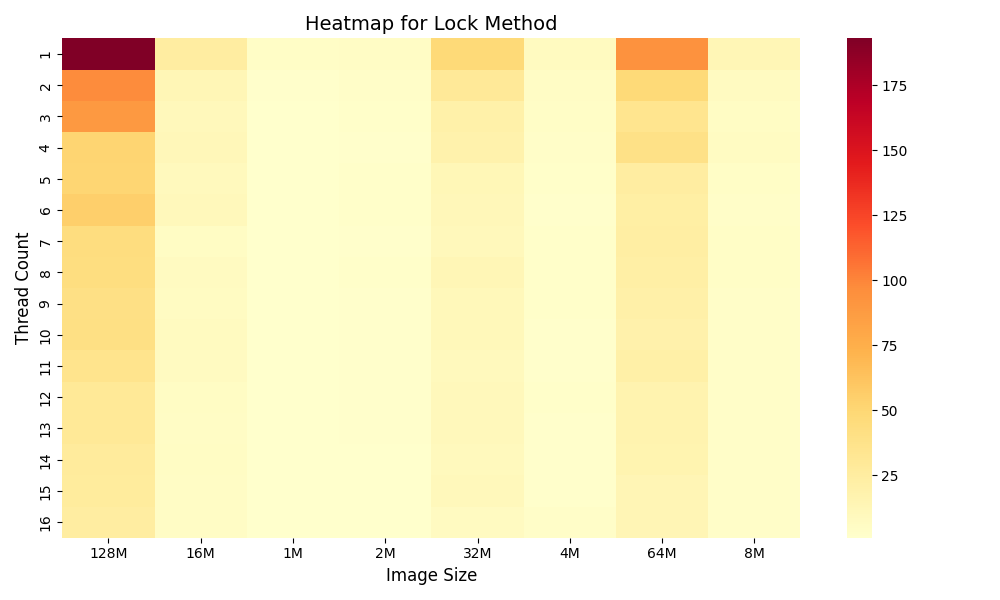
\includegraphics[width=.9\textwidth]{./figure/result2-Lock.png}
			\caption{Lock结果热力图}
		\end{subfigure}
		\begin{subfigure}{.32\textwidth}
			\centering
			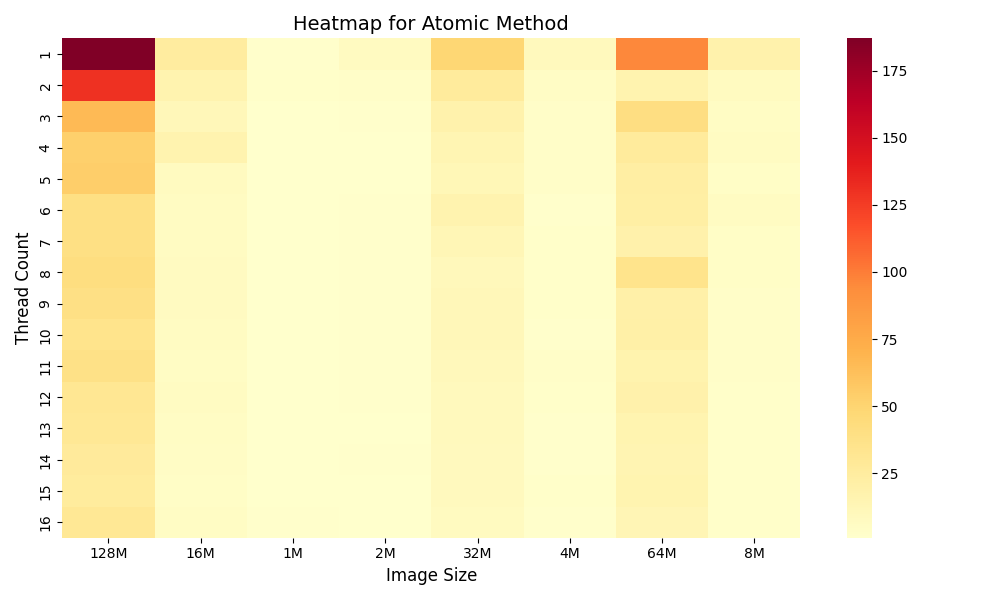
\includegraphics[width=.9\textwidth]{./figure/result2-Atomic.png}
			\caption{Atomic结果热力图}
		\end{subfigure}
		\begin{subfigure}{.32\textwidth}
			\centering
			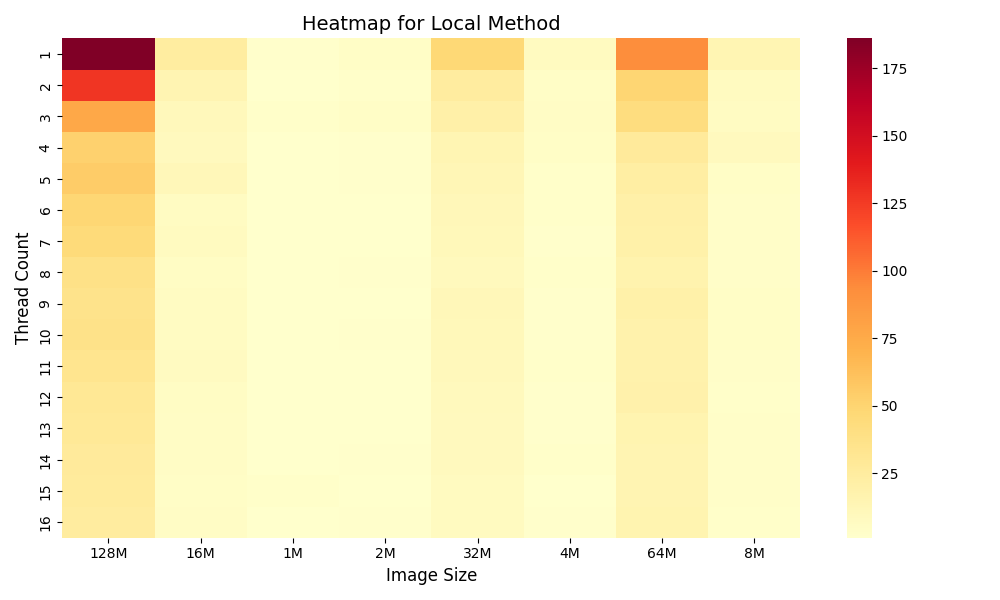
\includegraphics[width=.9\textwidth]{./figure/result2-Local.png}
			\caption{Local结果热力图}
		\end{subfigure}
		\caption{并行数组求和实验结果热力图}
	\end{figure}
	
	\section{总结与思考}
	
	\subsection{实验总结}
	
	本实验围绕 Pthreads 多线程编程技术,完成了两个核心任务:并行矩阵乘法与并行数组求和。在矩阵乘法部分,通过将行与列分配给多个线程并行处理,显著提升了大矩阵运算时的计算效率,验证了数据划分策略与线程数量对性能的敏感性。在数组求和部分,我们实现并比较了三种常用同步机制:基于锁的全局累加(Lock)、基于原子操作的累加(Atomic)以及每线程本地求和后统一归并的方式(Local)。从实验结果可以看出,随着数据规模的增大,Local 方法在性能上表现出明显优势,尤其在大于 8M 的数组中,能有效规避锁与原子操作带来的竞争开销,而 Lock 和 Atomic 方法则由于频繁的同步操作导致性能瓶颈。此外,线程数的变化也对不同方法的效率造成影响,合理的线程数选择与算法策略匹配成为提升多线程程序性能的关键。
	
	\subsection{实验心得}
	
	通过本次实验,我不仅深入理解了 Pthreads 的基本用法,如线程创建、同步与通信机制,还深刻体会到并行计算中“同步开销”对性能的重大影响。以数组求和实验为例,尽管 Lock 与 Atomic 实现较为直观,但在高并发场景下容易因锁竞争或内存一致性问题导致效率下降。而 Local 方法则展现了并行程序中“减少共享、增加局部”的优化思想,为今后设计高效多线程程序提供了实用的思路。此外,在调试多线程程序过程中,我也深刻体会到了线程调度的不确定性,意识到正确性保障机制的重要性。本实验提升了我分析性能瓶颈、选择合理并行策略的能力,同时也增强了我对系统资源调度、并发程序设计与调优的实际操作经验。
	
	\let\cleardoublepage\clearpage
	
	\begin{thebibliography}{99}  
		\bibitem{ref1} 彼得·S·帕切科,\ 马修·马伦塞克.\ 并行程序设计导论[M].\ 黄智濒,\ 肖晨\ 译.\ 原书第2版.\ 北京:机械工业出版社,\ 2024.
		\bibitem{ref2} 黄聃.\ 课件5[EB/OL].\ [2025-3-10].\ https://easyhpc.net/course/221/lesson/1416/material/3173.
	\end{thebibliography}
	
\end{document}
